\title{Absorption and Fluorescent Behavior in Ruby Crystal}

\author{William Cutler, Jack Donaghue, Haridas Kumarakuru, Don Heiman}

\newcommand{\abstractText}{\noindent
The unique optical properties of the ruby crystal that make it effective as a lasing medium were measured using a simple optical setup. Ruby’s absorption of visible light was shown to be strongest at \SI{420}{\nm} and \SI{550}{\nm}, corresponding to its physical appearance as translucent and pink. While the ruby crystal was illuminated with a \SI{532}{\nm} green laser, the R-line fluorescence peaked at \SI{693.8\pm1.1}{\nm}. Finally, the fluorescence lifetime of ruby was measured by pulsing the laser with a signal generator and capturing the decaying light waveform on a digital oscilloscope via a high-speed photodiode. An exponential decay time-constant of \SI{3.6\pm0.1}{\ms} was obtained. 
}

%%%%%%%%%%%%%%%%%
% Configuration %
%%%%%%%%%%%%%%%%%

\documentclass[11pt, a4paper, twocolumn]{article}
\usepackage{xurl}
\usepackage[comma, sort&compress]{natbib}
\usepackage{abstract}
\usepackage[separate-uncertainty=true]{siunitx}
\usepackage{graphicx}
\renewcommand{\abstractnamefont}{\normalfont\bfseries}
\renewcommand{\abstracttextfont}{\normalfont\small\itshape}
\usepackage{lipsum}

% Any configuration that should be done before the end of the preamble:
\usepackage{hyperref}
\usepackage{float}
\hypersetup{colorlinks=true, urlcolor=blue, linkcolor=blue, citecolor=blue}
\usepackage[a4paper, total={7in, 10in}]{geometry}
\setlength{\columnsep}{24pt}
\begin{document}
%%%%%%%%%%%%
% Abstract %
%%%%%%%%%%%%

\twocolumn[
  \begin{@twocolumnfalse}
    \maketitle
    \begin{abstract}
      \abstractText
      \newline
      \newline
    \end{abstract}
  \end{@twocolumnfalse}
]

%%%%%%%%%%%
% Article %
%%%%%%%%%%%

\section*{Introduction}
The absorption and fluorescence emission spectra have long been used to identify, characterize, and study materials \cite{BrittanicaSpectroscopy}. In lasing mediums such as ruby, these properties govern its excitation and emission spectra respectively. Studies of ruby absorption typically use a spectrophotometer and measure two broad absorption peaks centered near \SI{410}{\nm} and \SI{550}{\nm} \cite{Esposti,Kusuma,Song}. Devices with high resolution (\SI{0.5}{\nm} slit width) additionally detect a small doublet absorption peak near \SI{694}{\nm}. Song et. al. find absorption peaks at \SI{410}{\nm} and \SI{550}{\nm}, and calculates an absorption coefficient from these values according to Beer-Lambert's law.

The room temperature fluorescence spectrum of ruby has been reported well throughout the early 1900's with a double peak at \SI{692.7}{\nm} and \SI{694.2}{\nm}, corresponding to the characteristic $R_1$ and $R_2$ lines \cite{Kumari, Mani}. With lower resolution instruments, only a single primary peak was detected at \SI{694.2}{\nm} by Esposti et. al. Other fluorescence lines have been detected near these peaks at 671, 688, 695, and \SI{710}{\nm} \cite{Kusuma}, as the wavelengths can depend on the Cr concentration and impurity elements.

The effectiveness of ruby as a lasing medium depends on its ability to maintain a population inversion between the ground state and the meta-stable state. The stability of this meta-stable state can be measured by the fluorescence lifetime, which relates to how long the crystal will fluoresce in the absence of pumping, and therefore the time for which there is a size-able meta-stable population. Whereas most materials have nano or picosecond fluorescence lifetimes \cite{Berezin}, ruby’s fluorescence lasts milliseconds, and long enough to hold a population inversion for a working laser.

\begin{figure}
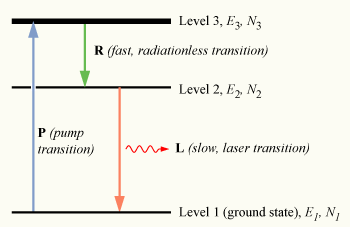
\includegraphics[width=\linewidth]{Population-inversion-3level.png}
\caption{\textit{Sample energy level diagram showing three phases of fluorescence: pumping, non-radiative relaxation, and fluorescent relaxation.}}
\label{fig:populationInversion}
\end{figure}

The fluorescence lifetime of around \SI{3.5}{\ms} is typically reported, but this measurement is dependent on a number of factors. Investigations of the temperature dependence show that lifetime decreases for temperatures above room temperature \cite{Seat, Nelson}. Investigations of the dependence on ruby diameter show an increasing fluorescence lifetime with increased size as emitted photons are reabsorbed more frequently in larger samples \cite{Jones}. The doping concentration can also effect the lifetime \cite{Brown}. Brown found that at room temperature, doping concentrations between 0.005\% and 0.1\% yielded lifetimes in the range of 3-\SI{4}{\ms}.

Many investigations use a single-exponential fit to obtain the fluorescence lifetime, but others use a double-exponential fit based on theoretical knowledge and the shape of the residuals for single-exponential fits \cite{McBane, Jones}. There is also some variation on whether a precise background constant is accounted for.

\section*{Experimental Setup}

A diagram of optical setup is shown in Figure 2, and Figure 3 shows the ruby crystal mounted on a post. For absorption measurements, white light from a Maglite was sent onto the crystal and the transmitted light was captured by a fiber optic, which was then sent to the spectrometer. The ruby mount was not fixed to the table, so that it could be moved out of the path of the white light in order to capture the unabsorbed light. Note that the flashlight must have a wide-spectrum incandescent bulb rather than a narrow-band LED.

\begin{figure}[]
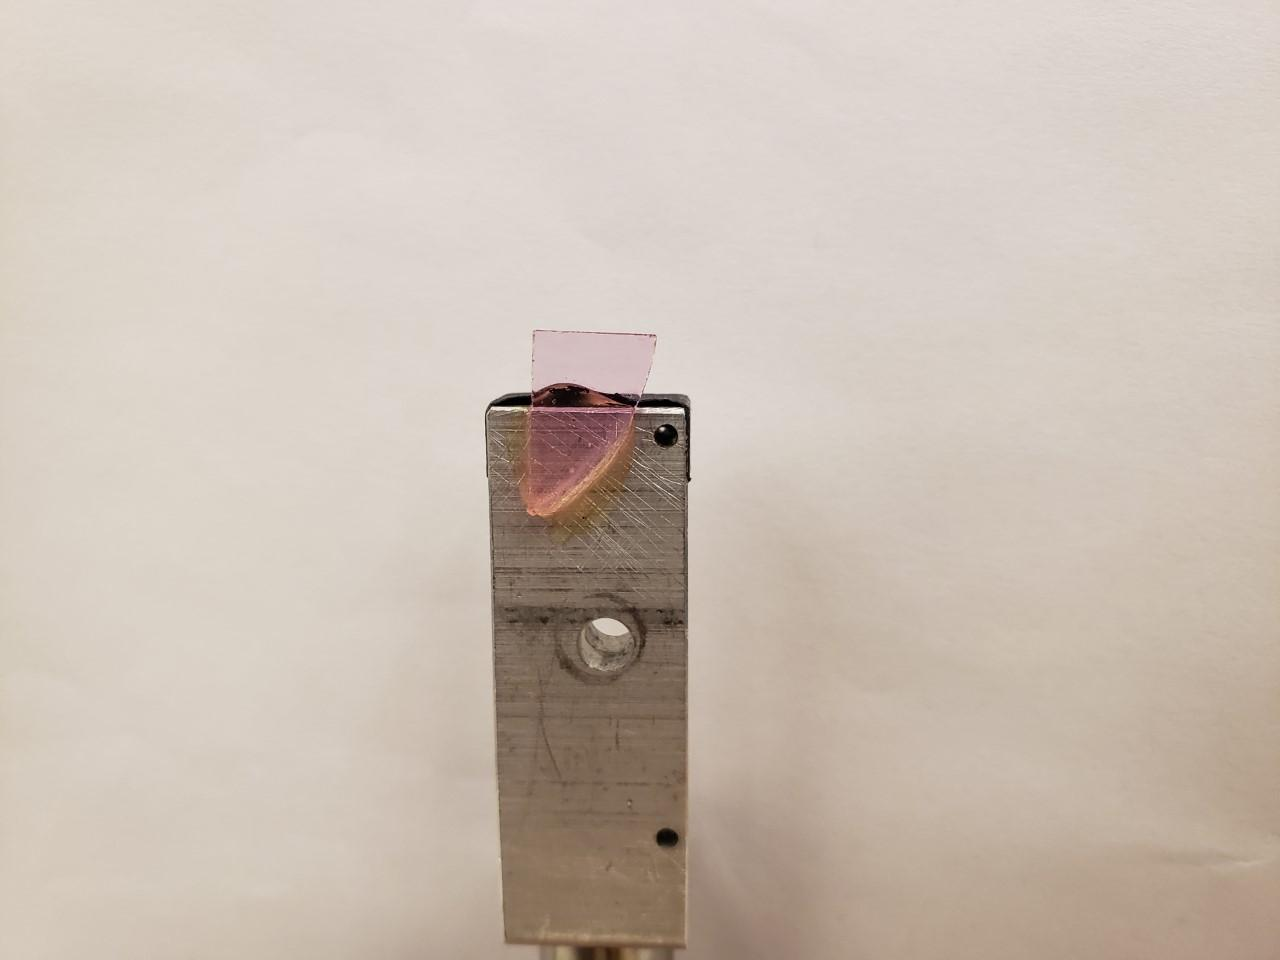
\includegraphics[width=\linewidth]{rubyPhoto.png}
\caption{\textit{Photograph of the transparent pink ruby crystal used throughout this study. Lasers and lights were directed to the top part of the crystal, above the metal stand.}
}
\label{fig:intensities}
\end{figure}

For fluorescence measurement, initial alignment began by positioning the fiber optic mount and focusing lens. A white light was placed at the end of the fiber optic such that its light would pass through the fiber, through the lens, and appear on the ruby sample. Adjustments to the mount and collection lens were made until this light was maximally focused on the ruby, since that would imply the fluoresced light is focused on the fiber optic mount. Additionally, the laser was briefly turned on during this adjustment to observe that the focused white light and laser both struck the ruby at the same location. These steps ensured that the fluoresced light that reached the fiber optic was powerful enough to be detected by the spectrometer.

\section*{Results}
\subsection*{Transmission and Absorption}

The transmittance of a material, $T$, is simply the fraction of incident light energy (or intensity) that passes through the material:
\setlength{\abovedisplayskip}{8pt}
\setlength{\belowdisplayskip}{8pt}
$$T=I/I_0$$.
$I_0$ represents the incident intensity, and was measured as a function of wavelength by shining a white light into the spectrometer at a particular distance. $I$ is the transmitted intensity, measured using exactly the same setup as $I_0$, but with the ruby crystal in the path between the light and the spectrometer. A black cloth ensured no interference from background light. Figure 4 shows the spectra of I and Io. Note that there is a larger difference in I and Io between 500 and 600 nm, which indicates an absorption peak in that region. That peak is clearly seen in the transmission spectrum in Figure 5.

\begin{figure}[H]
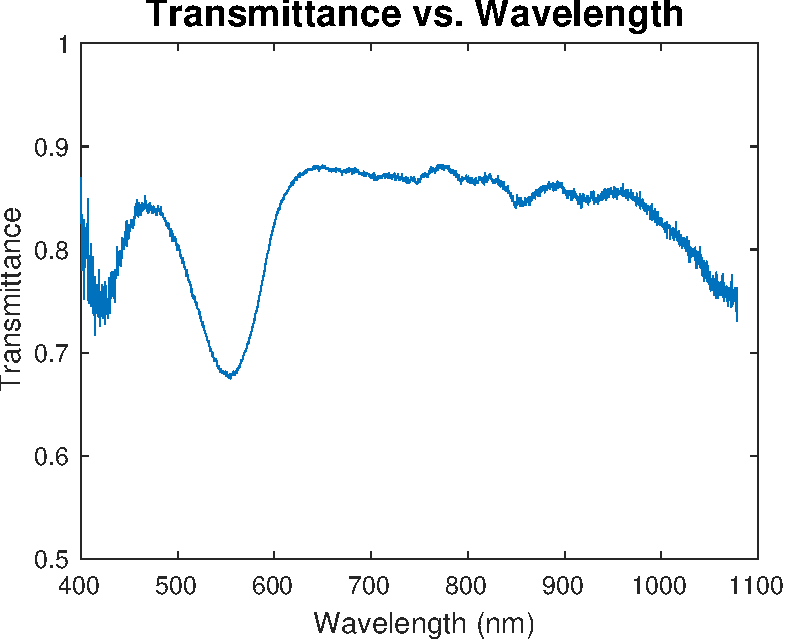
\includegraphics[width=\linewidth]{transmissionSpectrum.pdf}
\caption{\textit{Transmission spectrum of the ruby crystal showing prominent minima at 420 nm and 550 nm.}}
\label{fig:intensities}
\end{figure}

The reflectivity of the ruby is given by the formula below, and represents the proportion of incident light reflected at one ruby-air interface.
$$R=\frac{(n-1)^2}{(n+1)^2}$$
The reflectivity can be calculated using a value of $n = 1.780 \pm 0.018$. From these quantities, the absorption coefficient (of the exponential decay of light intensity as it travels along the length of the material) was calculated using:
$$ \alpha = \frac{1}{L}\ln(\frac{I}{I_0}(1-R)^2)$$.
Where $L$ is the length of the ruby measured along the path of the light passing through it (thickness). Below are the relevant quantities for calculating the absorption:
\\\\
\begin{tabular}{ll}
\textbf{Index of Refraction} & \textbf{1.78 ± 0.02}    \\
\textbf{Reflectivity}        & \textbf{7.58 ± 0.11\%}  \\
\textbf{Length}              & \textbf{2.00 ± 0.05 mm}  
\end{tabular}
% \begin{figure}[H]
% 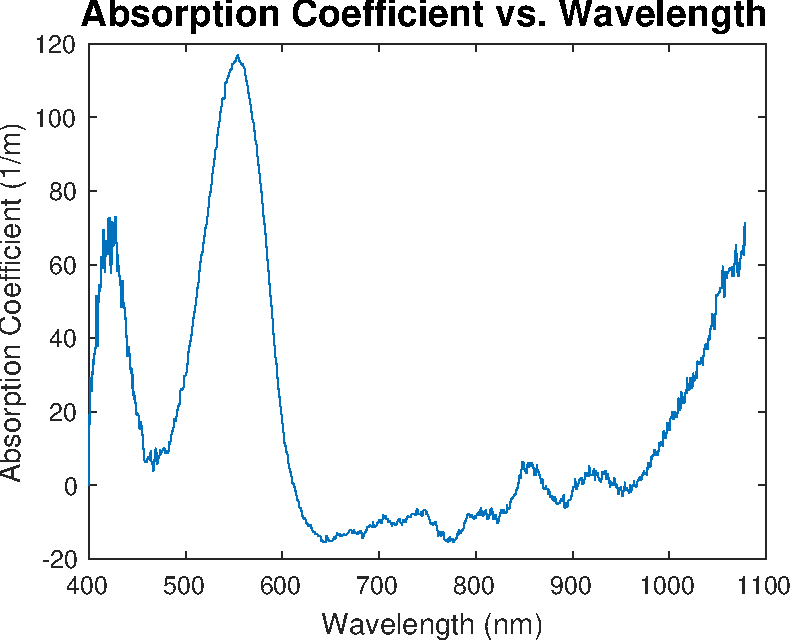
\includegraphics[width=\linewidth]{absorptionSpectrum.pdf}
% \caption{Absorption spectrum of the ruby crystal with two absorption peaks centered at 410 nm and 550 nm}
% \label{fig:intensities}
% \end{figure}

\begin{figure}[]
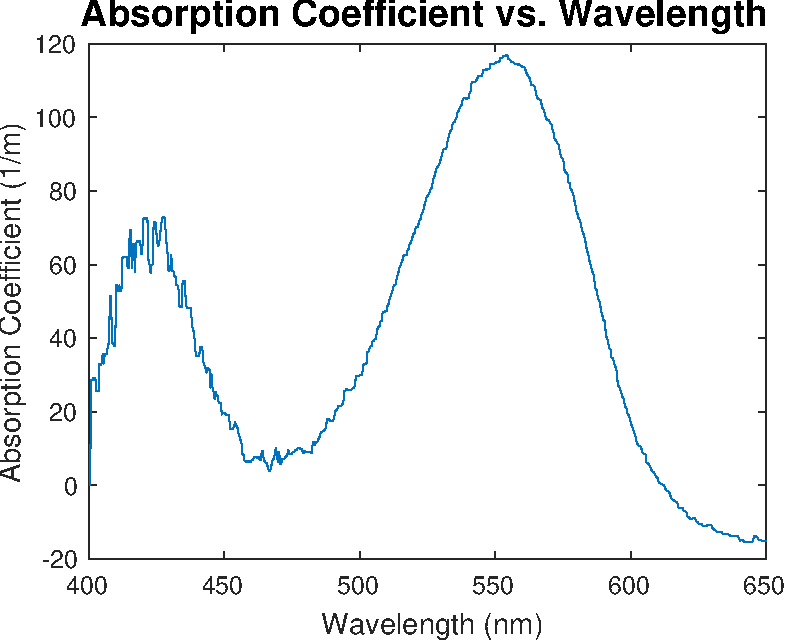
\includegraphics[width=\linewidth]{absorptionSpectrumFocused.pdf}
\caption{\textit{Absorption spectrum of a ruby crystal showing two broad absorption peaks centered at 410 nm and 550 nm.}}
\label{fig:intensities}
\end{figure}

% \begin{figure}[]
% 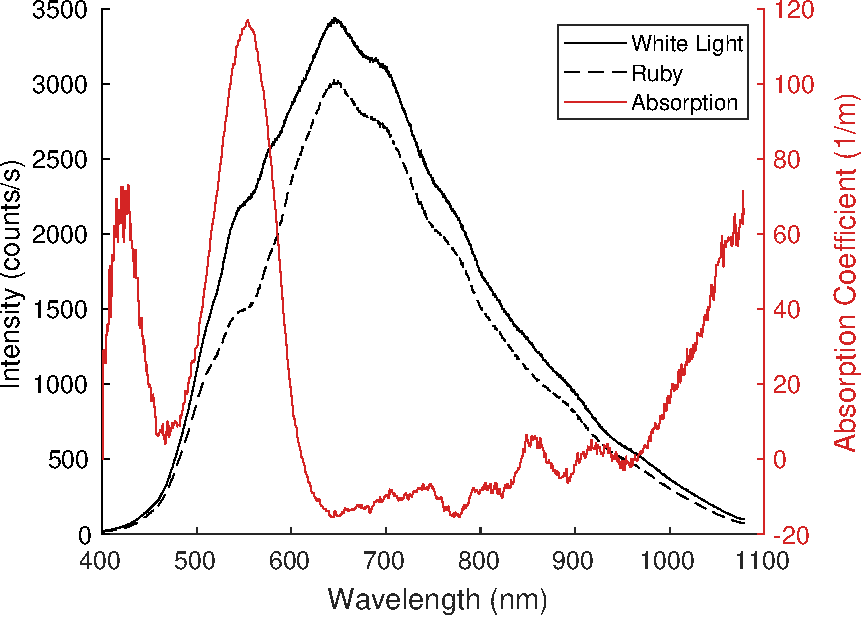
\includegraphics[width=\linewidth]{absorptionAndIntensitySpectra.pdf}
% \caption{\textit{Combination of intensity and absorption spectra showing a correspondence between the strongest absorption peak and intensity differential between measurements with and without ruby.}

% \label{fig:intensities}
% \end{figure}

\begin{figure}[]
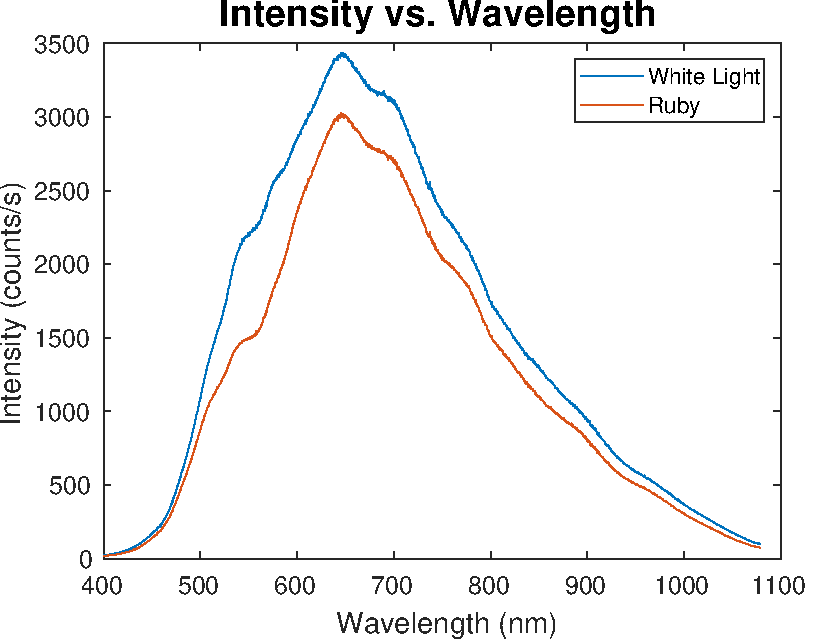
\includegraphics[width=\linewidth]{doubleIntensityMeasurement.pdf}
\caption{\textit{Spectrum of intensities for bare white light and white light passing through ruby.}
}
\label{fig:intensities}
\end{figure}

Because transmittance was recorded as a function of wavelength and other quantities are constant, the absorption coefficient is also a function of wavelength, yielding an absorption spectrum, shown in Figure 6. The absorption has broad peaks at 420 ± 5 nm and 553 ± 1 nm wavelengths. These corresponded to absorption coefficients of 66.5 ± 9.9 m$^{-1}$ and 116.7 ± 1.1 m$^{-1}$, respectively. With these values, the intensity of the light would be expected to be reduced by a factor of e after traversing 15 ± 2 mm and 8.57 ± 0.08 mm respectively. That these lengths are much greater than the actual thickness of the ruby crystal is consistent with the fact that it is mostly transparent. The pink color of the ruby crystal is due to the broad absorption bands of Cr$^{3+}$ in the violet (400 - 450 nm) and yellow-green (500 - 600 nm) regions, with a minimum of absorption in the deep red region ($>$ 650 nm).

\subsection*{Fluorescence Spectrum}

Peak R-Line fluorescence occurred at 693.5 nm, a deep red color, with a 8 nm FWHM for the entire peak, shown in Figure 7. A streak of red light could be seen by looking down into the top of the ruby crystal. Because the spectrometer used had a resolution of $>$1 nm, it was unable to discern the double peak found in other experiments, instead showing a single peak spanning the entire double peak range 692.7 to 694.3 nm. Also captured by the spectrometer are smaller peaks on either side of the primary R-line, at 670 nm and 710 nm, corresponding to neighbor (N) lines and side bands, respectively, as detected by Kusuma \cite{Kusuma}.
% \begin{figure}[H]
% 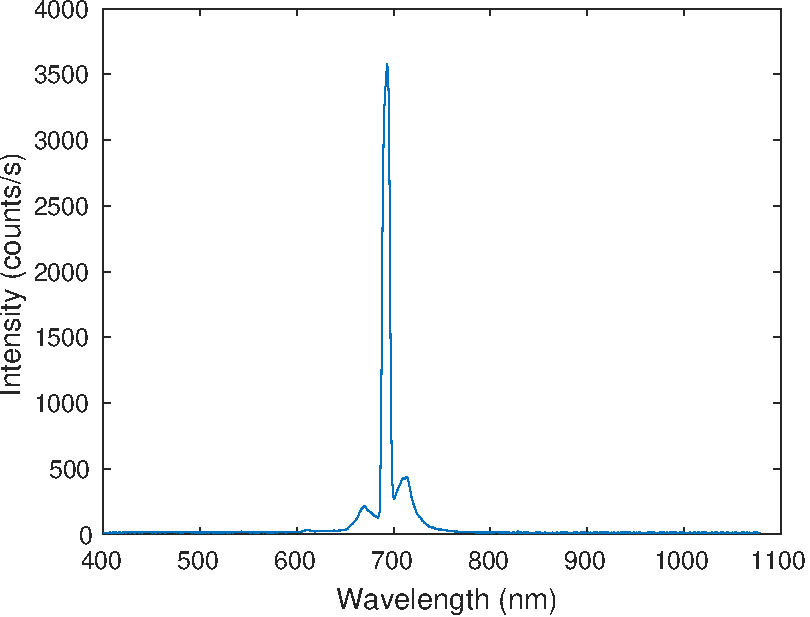
\includegraphics[width=\linewidth]{fluorescenceSpectrum.pdf}
% \caption{Fluorescence spectrum resulting from 532 nm excitation laser showing R-line fluorescence at 693.5 nm}
% \label{fig:intensities}
% \end{figure}
\begin{figure}[]
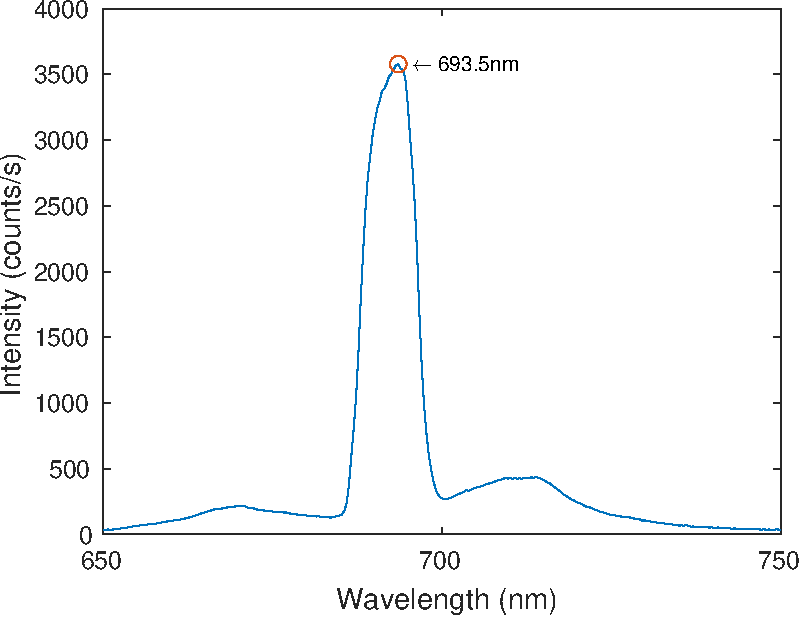
\includegraphics[width=\linewidth]{fluorescenceSpectrumFocused.pdf}
\caption{\textit{Fluorescence spectrum of a ruby crystal showing fluorescence near the R-line peak.}}
\label{fig:intensities}
\end{figure}

\subsection*{Fluorescence Lifetime}
Important aspects of the fluorescence process were observed by measuring the strength of fluorescence across time for a ruby crystal subjected to a pulsed laser. The diagram in Figure 8 illustrates the setup and signal path. The laser was pulsed by a 10 Hz square wave function generator and the ruby fluorescence was captured by a photo-diode. The two-channel oscilloscope simultaneously recorded the square wave that pulsed the laser (yellow arrow) and the fluorescence signal captured by the photo-diode (blue arrow). A photograph of the optical bench for this process is shown in Figure \ref{fig:laserBenchPhoto}.
\begin{figure}[]
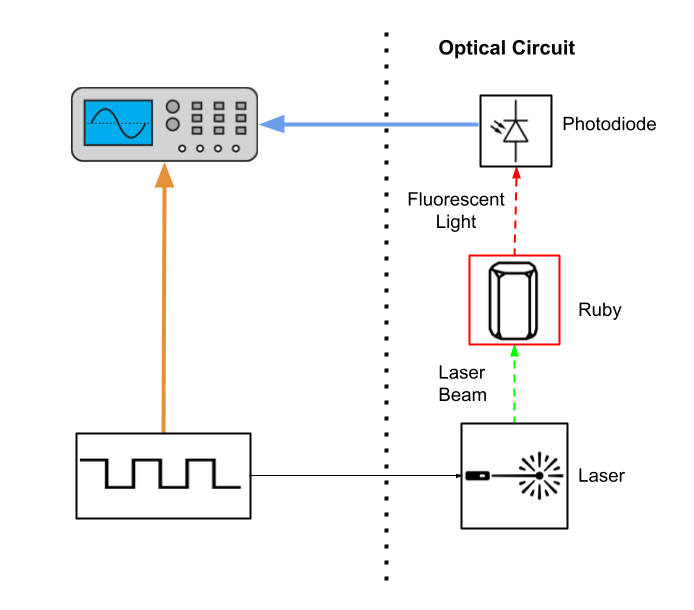
\includegraphics[width=\linewidth]{decayMeasurementSchematic.png}
\caption{\textit{Schematic illustration of fluorescence lifetime measurement showing how the square-wave electrical signal of the laser and fluorescence input to the oscilloscope.}}
\label{fig:decayMeasurementSchematic}
\end{figure}

\begin{figure}[]
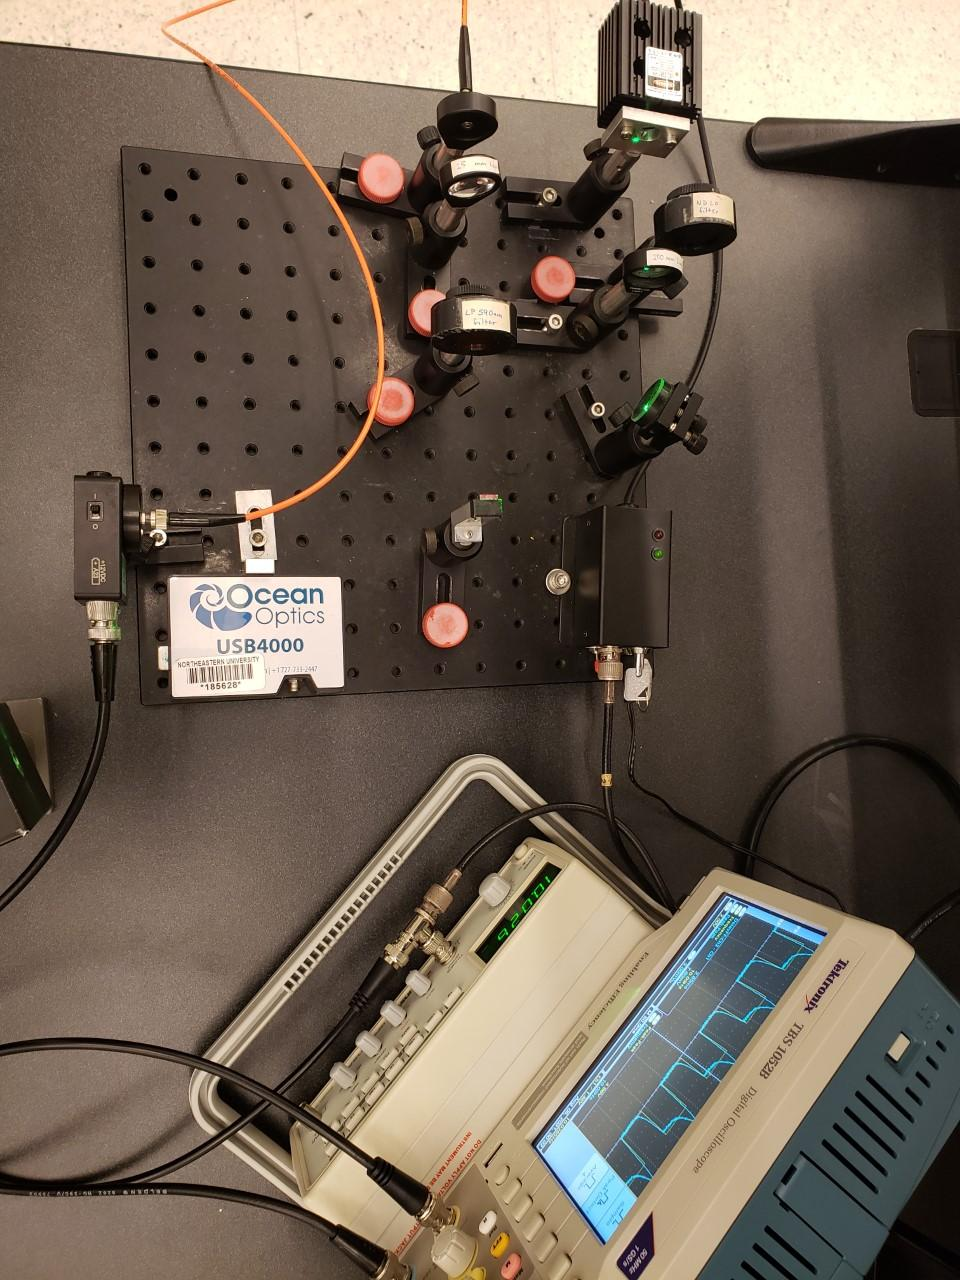
\includegraphics[width=\linewidth, height=\linewidth]{laserBenchPhoto.png}
\caption{\textit{Photograph of laser bench setup for measuring fluorescence lifetime.
}}
\label{fig:laserBenchPhoto}
\end{figure}

The oscilloscope captured one period of the 10 Hz signal as shown in Figure 10, with the square  wave  in  blue  and  the  fluorescence  in  orange. 
It shows a series of distinct phases outlining the entire process of fluorescence. The fluorescence rises sharply t = 0.015 to 0.025 s, as chromium ions fluoresce back to the ground state. From t = 0.025 s until the laser pulse turns of at t = 0.05 s the fluorescence is constant, as the rates of emission and excitation are equal. Finally, after t = 0.05 s, with the laser turned off, fluorescence continues, and the rate of fluorescence decreases exponentially. The rate of this exponential decay is governed by the probability that a given metastable chromium atom will fluoresce and relax in a given period of time. 

\begin{figure}[]
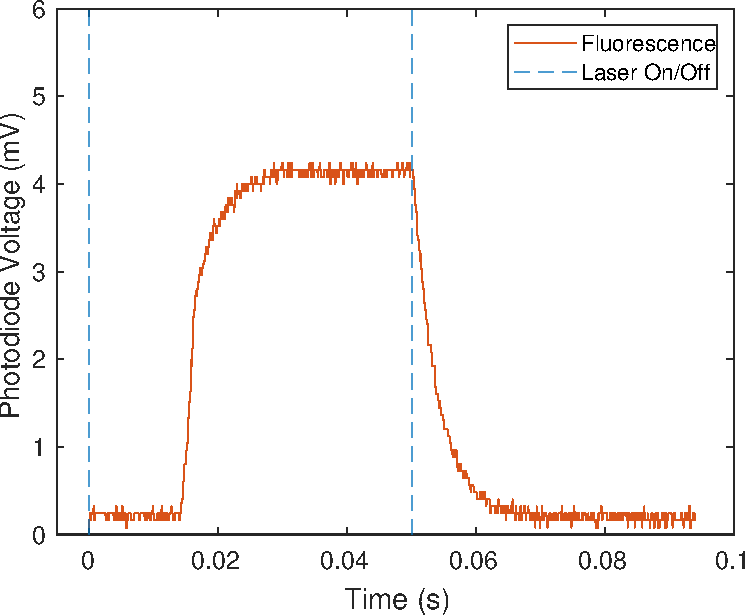
\includegraphics[width=\linewidth]{fluorescencePeriod.pdf}
\caption{\textit{Oscilloscope traces for one period of laser pulse at 10 Hz, showing the fluorescence emission in red and the laser excitation in blue that ends at 0.05 s.}}
\label{fig:fluorescencePeriod}
\end{figure}

The fluorescence decay was isolated from the oscilloscope data, and a single exponential fit of the form $y = ae^{-x/\tau} + c$ was applied to determine the  lifetime tau = 3.6 +- 0.1 ms, as shown in Figure 11. The inclusion of a constant in the fit was important because the photodiode voltage does not decay to 0, but has a small background value below 0.5 mV.

\begin{figure}[]
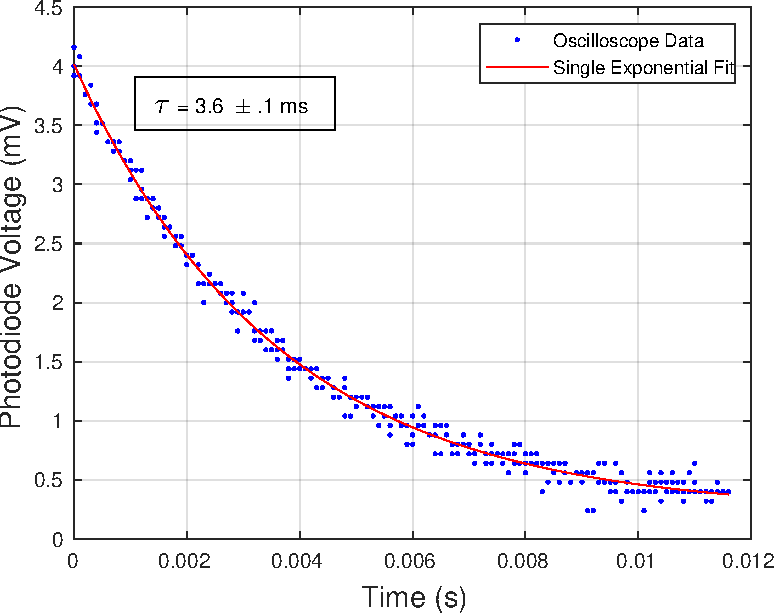
\includegraphics[width=\linewidth]{decayFit.pdf}
\caption{\textit{R-line fluorescence data as a function of time in blue points. The red curve is a MATLAB fit to the data.}
}
\label{fig:populationInversion}
\end{figure}

A single-exponential fit is reported here for its simplicity and interpretability. Furthermore, it provided a high correlation ($R^2 = .993$), and its residual plot, shown in Figure \ref{fig:decayResiduals}, has no discernible pattern, unlike those reported by \cite{Jones} in justification of the double exponential. This is not to deny the theoretical relevance of a double exponential to describing the fluorescence process, but rather to demonstrate that the single exponential fits the data remarkably well beyond mere visual inspection.

\begin{figure}[]
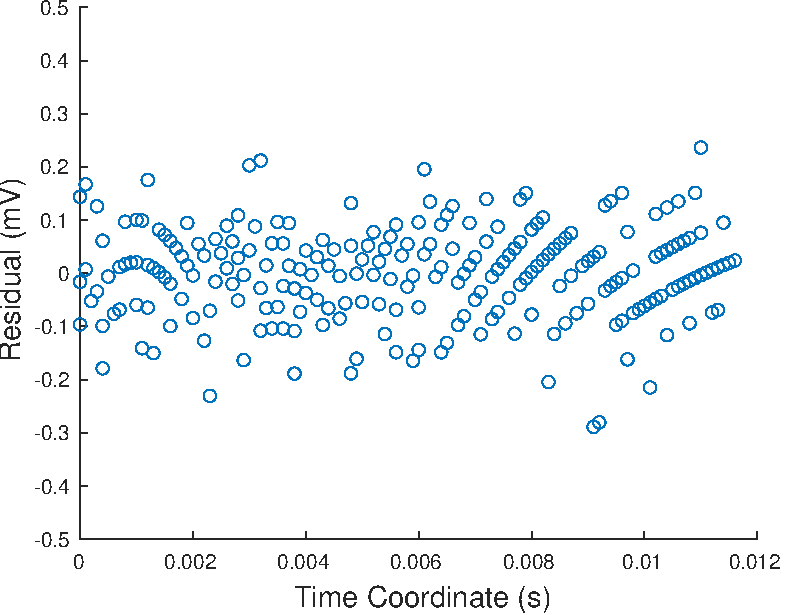
\includegraphics[width=\linewidth]{decayResiduals.pdf}
\caption{\textit{Residual plot for the single exponential fit to the fluorescence data in the previous figure, showing no discernible pattern that might indicate a more complex fit is needed.}}
\label{fig:decayResiduals}
\end{figure}

The time constant represents the amount of time for the fluorescence decay rate to decrease to 1/e of its original value. Whereas many materials exhibit fluorescence lifetimes on the order of ns or ps, ruby’s fluorescence lasts multiple milliseconds, and is a significant factor in its effectiveness as a lasing medium.

\section*{Discussion}
The the experiments and analysis performed concern the optical properties of the ruby crystal sample. The absorption spectrum was found to have peak absorptions at wavelengths of 420 ± 5 nm and 553 ± 1 nm with absorption depths of 15 ± 2 mm and 8.57 ± 0.08 mm, respectively. The transmission and absorption spectra of the ruby were consistent with its visual appearance as a pink translucent crystal. The fluorescence showed a singular clear peak at 693.5 ± 1.1 nm. This range would encompass the double line of the ruby fluorescence spectrum at 692 and 694 nm recorded by (cite source). The R-Line fluorescence lifetime was found to be equal to 3.6 ± 0.1 ms.

The results of the experiment would be affected by light from the laboratory if the black cloth used to cover the optic setup were to allow a small amount of light to enter the setup and affect the collected light. Also any dust, oil, or other impurities touching the laser, ruby, spectrometer, or optical component would likewise have changed the measurements and introduced sources of error.

\subsection*{Acknowledgements}
We would like to thank Nathaniel Avish and Hongwei Chen, for their help in the laboratory and as teaching assistants for the Advanced Physics Laboratory section for which this experiment was introduced. We would also like to thank the Northeastern University Department of Physics for supporting our experience at the conference financially.
%%%%%%%%%%%%%%
% References %
%%%%%%%%%%%%%%

\nocite{*}
\bibliographystyle{unsrt}
\bibliography{reference}

\end{document}

